\section{Results}
In this section we perform let the Q-learning algorithm act on the previously defined environments. To ensure that the learning algorithm explores the state space we will use an $\eps$-greedy algorithm, if not stated otherwise. The decay of the epsilon greedy algorithm will be linear with the number of episodes has passed one tenth of the number of simulations. As an example, if we perform $10^6$ simulations then after a fixed point the proability of taking a random action will decay by $1 / \text{episode}$. Also, the initial values of $Q(S, a)$ will be zero for all states $S$ and actions $a$. 

Two state space representations will be used in this section. These are $(\mathbf{X}_p, \sum_d)$ and $(\sum_p, UA, , \sum_d)$ which henceforth will be called ''hand''- and ''sum''- environments or state spaces. For visualisations we will aggregate the results of the Q-learning algorithm on the hand environment to a sum representation.

In Figure \ref{fig:avg_return} we can see the average return by episodes, when the Q-learning algorithm is acting on different environments. Both algorithms seem to have a negative trend in the first episodes. This is to be expected since the $\eps$ greedy assures that we explore the state space in the first iterations. In $\eps$ number of cases we aim  

\begin{figure}[htp]
 \centering
	 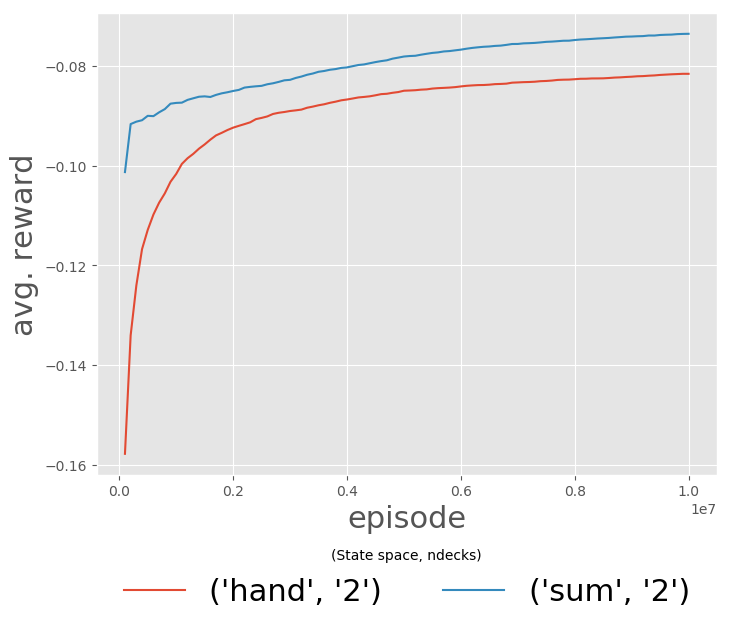
\includegraphics[scale=0.7]{./figures/avgReturnEp_ndeck2.png}
 % .: 0x0 pixel, 0dpi, 0.00x0.00 cm, bb= width=0.9\linewidth, 
 \caption{The average return of an $\epsilon$-greedy Q-learning algorithm for TEST different state spaces. \label{fig:avg_return}}
\end{figure}



In Figure \label{fig:avg_return_sums}, something happens where something is supposed to happen. 

\begin{figure}[htp]
\centering
 \begin{subfigure}[b]{0.3\textwidth}
  	 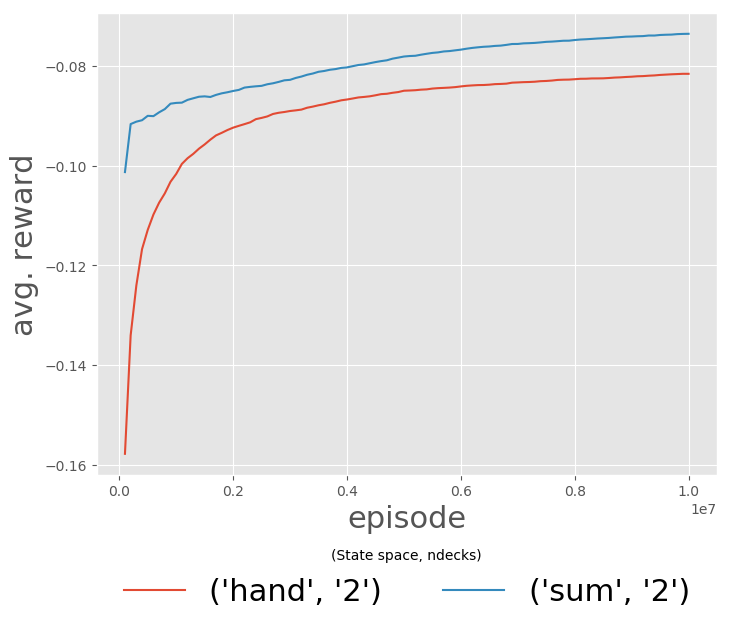
\includegraphics[width=\textwidth]{./figures/avgReturnEp_ndeck2.png}
   % .: 0x0 pixel, 0dpi, 0.00x0.00 cm, bb=
   \caption{The average return of an $\epsilon$-greedy Q-learning algorithm for TEST different state spaces. \label{fig:avg_return_sums}}
 \end{subfigure}
 \hspace{0.2cm}
 \begin{subfigure}[b]{0.3\textwidth}
  	 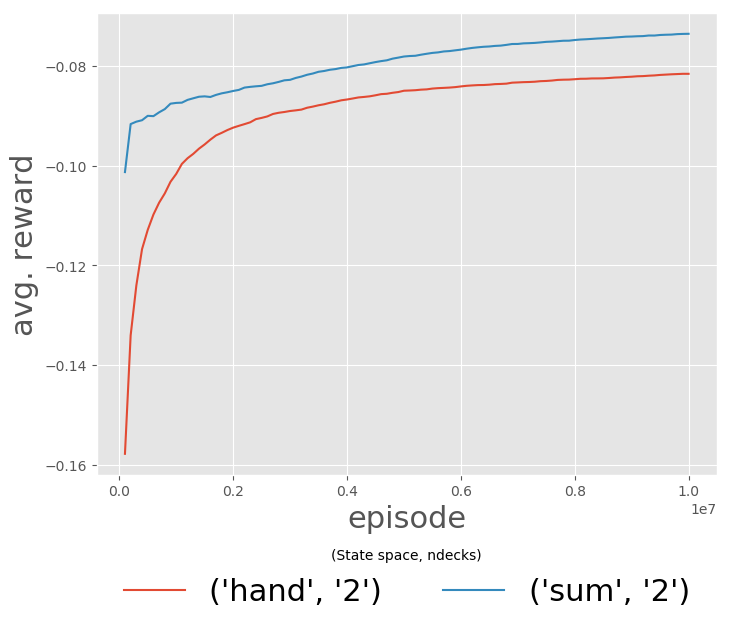
\includegraphics[width=\textwidth]{./figures/avgReturnEp_ndeck2.png}
   % .: 0x0 pixel, 0dpi, 0.00x0.00 cm, bb=
   \caption{The average return of an $\epsilon$-greedy Q-learning algorithm for TEST different state spaces. \label{fig:avg_return_sums}}
 \end{subfigure}
\end{figure}